% -*- mode: LaTeX; mode: TeX-PDF; coding:utf-8 -*-


\label{sec:func_recv_intro}

\emph{Практическое значение восстановления многомерных данных тут дб более широкое.}
Задачи восстановления данных возникают в разных областях обработки информации,
в том числе в задачах прикладной гидроакустики. 

% \emph{Например.}
% Задача восстановления данных 
% %функции нескольких переменных 
% по 
% %ее 
% известным значениям
% в узлах некоторой сетки имеет большое практическое %прикладное 
% значение. Ее часто приходится
% решать как самостоятельную задачу, кроме того, она является элементом решения
% многих вопросов прикладного характера. %, в частности, цифровой обработки
% %многомерных сигналов. 


%\emph{
%%Одномерный случай
%Пусть известны значения некоторой функции $\varphi$
%в $K$ узлах $ u^{(k)}$, %($k = 0, \ldots, {K-1}$), 
%равномерно расположенных с шагом $h$.
%}

%Двумерный случай
%% ?? Общий: функции нескольких переменных
Пусть известны значения  функции $\varphi$, принадлежащей некоторому классу гладкости, 
в  узлах $\{u^{(k)}=kh\}$ ($k\in \mathbb{Z}_+^n$, $\mathbf{0}^n \le k \le K-\mathbf{1}^n$, $h>\mathbf{0}^n$, $K\in \mathbb{N}^n$) прямоугольной
равномерной сетки. 
Необходимо приближённо найти неизвестные значения
этой функции между заданными узлами (см. рисунок~\ref{fig:net_common}).
\begin{figure}[h!]
  \centering
  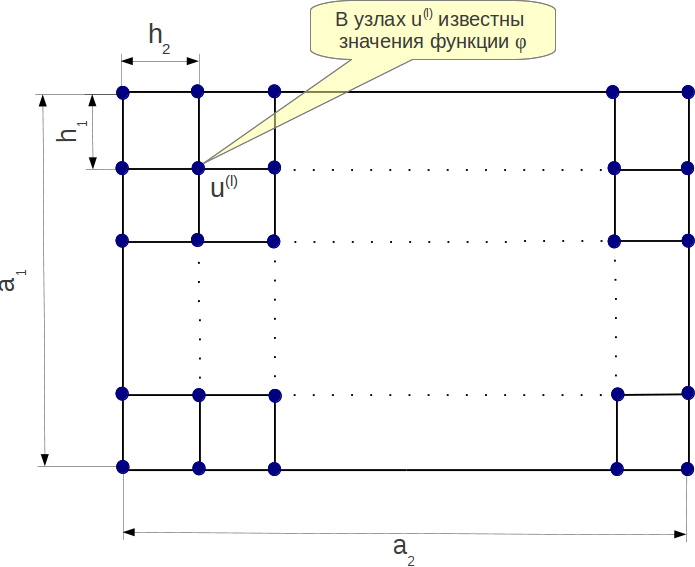
\includegraphics{net_2D}
  \caption{Постановка задачи}
  \label{fig:net_common}
\end{figure}
%\FloatBarrier
При этом, зачастую, необходимо обработать достаточно большие объёмы данных.
Представляется актуальным поиск и реализация эффективных параллельных алгоритмов
для решения описанной задачи.

% Рассмотрим случай, когда 
% узлы расположены на прямоугольной равномерной сетке.
% Пусть задан прямоугольник $\Pi$. Стороны прямоугольника 
% разбиваются на  равные части с шагами  $h_1$ и $h_2$ по каждой стороне соответственно.
% Обозначим $\boldsymbol{h} = (h_1,h_2)$.
% Узлы равномерной сетки 
% задаются следующим образом:
% $\{u^{(\boldsymbol{k})} = (k_1h_1,k_2h_2) \}$,
% %где $k_i$ целые числа, --- для более общего случая чем 2D можно так
% $\boldsymbol{k}=(k_1,k_2)$,
% где
% $k_1 = 0,\ldots,K_x$,
% $k_2 = 0, \ldots, K_y$,
% $K = K_x \times K_y$.
% В точках $u^{(\boldsymbol{k})}$ 
% известны значения функции $\varphi$.
% %Требуется найти гладкую на $\Pi$
% %функцию $g$ <<хорошо>> аппроксимирующую $f$.

Сетку с известными значениями в узлах будем называть \textit{крупной сеткой}.

В настоящей работе мы остановимся на вычислительных аспектах
решения задачи восстановления данных в многомерном случае. 
Считаем что, узлы
% $u^{(\boldsymbol{m})}$, 
%   $0*n \le \boldsymbol{m}=(m_1,m_2)$, 
$ \{v^{(m)}=mt\}$,  ($m\in \mathbb{Z}_+^n$, $\mathbf{0}^n \le m \le M-\mathbf{1}^n$,
$t>\mathbf{0}^n$ $M\in \mathbb{N}^n$), 
в которых требуется найти значения, 
также расположены
равномерно.
% Т.~е. 
% требуется вычислить значения 
% в $M = M_x \times M_y = K_x(N+1) \times K_y(N+1)$ узлах,
% равномерно расположенных по каждой оси,
% где $N$ --- произвольное натуральное число.
Такую  систему узлов %сетку размером %$M = N(K-1) + K$
будем называть
\textit{мелкой сеткой}.
% Обозначим для удобства $N^* = N+1$.
%В этих обозначениях количество узлов мелкой сетки $M = N^* (K-1) + 1$.



%Был выбран 
В работе рассматривается параллельная реализация
алгоритма,
%предложенный 
В.~В.~Жука~\cite{book_Zhuk},
обладающего низкой вычислительной сложностью
и хорошим потенциалом в смысле параллелизма по данным. 

\emph{Отображение массового параллелизма по данным на архитектуру GPU.}



%На его основе  
%построены эффективные параллельные алгоритмы в терминах модели
%блочно-синхронно-конвейерного параллелизма (БСКП),
%которая объединяет в себе модель вычислительной системы
%и формальное описание обработки потока данных в реальном времени,
%представленные в работе~\cite{my_paper_LETI_MCS}.

\emph{Обзор моделей применительно к GPU}
В настоящей работе развивается
хорошо изученный в литературе
(например, в работах~\cite{paper_Val_BSP_90, paper_BSPStreaming,  paper_McColl_Tis})
подход к проектированию
алгоритмов с применением моделей параллельных вычислений.


С другой стороны, отметим работу~\cite{paper_Mas_recv},
%\emph{а там многомерный случай??} 
где рассматриваются вопросы параллельной реализации
похожих алгоритмов восстановления данных.



%%% Local Variables: 
%%% mode: latex
%%% TeX-master: "paper_func_recv"
%%% End: 



